%%%%%%%%%%%%%%%%%%%%%%%%%%%%%%%%%%%%%%
%%%%%%%%%%%%%%%%%%%%%%%%%%%%%%%%%%%%%%
% Do not edit the TeX file your work
% will be overwritten.  Edit the RnW
% file instead.
%%%%%%%%%%%%%%%%%%%%%%%%%%%%%%%%%%%%%%
%%%%%%%%%%%%%%%%%%%%%%%%%%%%%%%%%%%%%%



The posterior quantities of interest in this application are the admixtures
$\pi_\n$. \figref{stru_init_fit} plots the inferred admixtures
$\expect{\q(\pi_\n \vert \etaopt)}{\pi_\n}$ for all individuals $\n$.

In the approximate posterior with $\alpha_0$, there appear to be three dominant
latent populations, which we arbitrarily label as populations 1, 2, and 3
(\figref{stru_init_fit}). The inferred admixture proportions generally
correspond with geographic regions: Mbololo individuals are primarily population
1; Ngangao individuals are primarily population 2; and Chawia individuals are a
mixture of populations 1, 2, and 3.


\begin{knitrout}
\definecolor{shadecolor}{rgb}{0.969, 0.969, 0.969}\color{fgcolor}\begin{figure}[!h]

{\centering 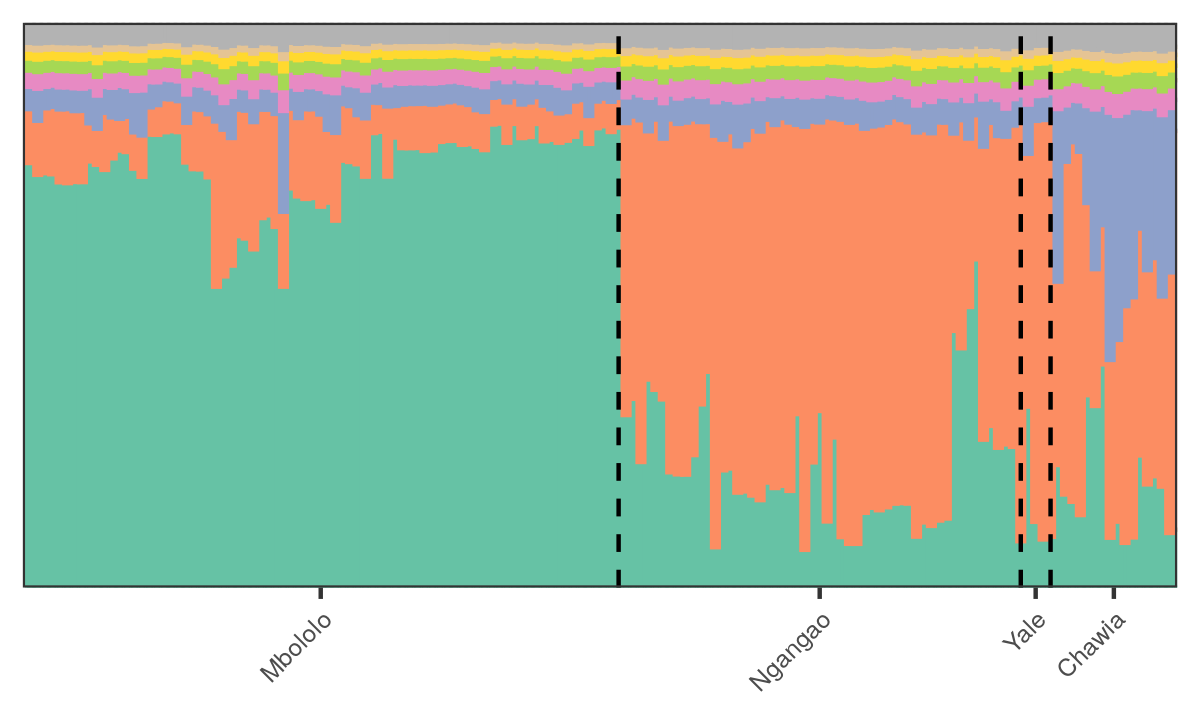
\includegraphics[width=0.980\linewidth,height=0.470\linewidth]{figure/stru_init_fit-1} 

}

\caption[The inferred individual admixtures at $\alpha_0 = 3$.
    Each vertical strip is an individual and each color
    a latent population.
    Lengths of colored segments represent the inferred admixture proportions.
    Individuals are ordered by the geographic region from which they were sampled
    (Mbololo, Ngangao, Yale, and Chawia).
    In the text, we refer to the green, orange, and purple latent populations
    as population 1, 2, and 3, respectively]{The inferred individual admixtures at $\alpha_0 = 3$.
    Each vertical strip is an individual and each color
    a latent population.
    Lengths of colored segments represent the inferred admixture proportions.
    Individuals are ordered by the geographic region from which they were sampled
    (Mbololo, Ngangao, Yale, and Chawia).
    In the text, we refer to the green, orange, and purple latent populations
    as population 1, 2, and 3, respectively. }\label{fig:stru_init_fit}
\end{figure}


\end{knitrout}
